\documentclass[11pt, addpoints, answers]{exam}

\usepackage{amsmath, amssymb, euler}
\usepackage{xcolor}
\usepackage{algorithm, algorithmicx, algpseudocode}
\usepackage{tikz, tikz-qtree, drawstack}
\usepackage[shortlabels]{enumitem}

\usetikzlibrary{graphs}
\tikzset{every tree node/.style={minimum width=2em,draw,circle},
	blank/.style={draw=none},
	edge from parent/.style=
	{draw,edge from parent path={(\tikzparentnode) -- (\tikzchildnode)}},
	level distance=1.2cm}

% For inserting code snippets.
\usepackage{listings}
\lstset{
    columns = fixed,
    basewidth = {0.5em},
    breaklines = true,
    backgroundcolor = \color{white},
    keywordstyle = \color[RGB]{40, 40, 255},
    numberstyle = \footnotesize\color{darkgray},
    commentstyle = \ttfamily\color{violet},
    basicstyle = \ttfamily,
    stringstyle = \ttfamily\color[RGB]{128, 0, 0},
    showstringspaces = false,
    language = {[11]C++},
    escapechar = \@
}
\lstnewenvironment{cpp}[1][]{\lstset{language = {[11]C++}, #1}}{}

\usepackage{tikz}

% headers, footers, titles
\newcommand{\CourseName}{CS101 Algorithms and Data Structures}
\newcommand{\HomeworkNO}{Homework 4}
\newcommand{\DueDate}{Due date: 23:59, October 16th, 2022}

\pagestyle{headandfoot}
\runningheadrule
\runningheader{\CourseName}{\HomeworkNO}{\DueDate}
\runningfooter{}{\thepage}{}

\title{
	\CourseName\\
	Fall 2022\\
	\HomeworkNO
}
\author{}
\date{\DueDate}

% formats of questions, choices, points, etc.
\qformat{\bf\thequestion. (\totalpoints\ points) \thequestiontitle\hfill}
\pointname{'}
\CorrectChoiceEmphasis{\bf\color{blue}}

% We frequently use this font.
\newcommand{\ttt}{\texttt}
\newcommand{\blue}[1]{\textcolor{blue}{#1}}
\newcommand{\bluett}[1]{\blue{\ttt{#1}}}

\begin{document}

\maketitle

\begin{enumerate}
	\item Please write your solutions in English.
	\item Submit your solutions to gradescope.com.
	\item Set your FULL name to your Chinese name and your STUDENT ID correctly in Account Settings.
	\item If you want to submit a handwritten version, scan it clearly. \ttt{CamScanner} is recommended.
	\item When submitting, match your solutions to the problems correctly.
	\item No late submission will be accepted.
	\item Violations to any of the above may result in zero points.
\end{enumerate}

\newpage


{\large\textbf{Notes}:}

\begin{enumerate}
	\item Some problems in this homework requires you to design Divide and Conquer algorithm. When grading these problems, we will put more emphasis on how you reduce a problem to a smaller size problem and how to combine their solutions with Divide and Conquer strategy. 
	\item Your answer for these problems {\color{red}\textbf{should}} include:
	\begin{enumerate}
		\item {\color{red}Algorithm Design}
		\item {\color{red}Time Complexity Analysis}
		\item Pseudocode (Optional)
	\end{enumerate}
    \item Your answer for these problems is {\color{red}not allowed to include real C or C++ code}.
	\item In Algorithm Design, you should describe each step of your algorithm clearly.
	\item Unless required, writing pseudocode is optional. If you write pseudocode, please give some additional descriptions if the pseudocode is not obvious.
	\item You are recommended to finish the algorithm design part of this homework with \LaTeX.
\end{enumerate}

\newpage

\begin{questions}


\titledquestion{Proving a problem in $\NPC$}[0]

When proving problem $A\in \NPC$, please clearly divide your answer into the following (1+2) sections:
\begin{enumerate}
	\item Show that $A\in \NP$.
	\item Choose a problem $B\in \NPC$ and show that $B\leq_p A$.
	      \begin{enumerate}
		      \item For every instance $I_B$ of $B$, construct an instance $I_A$ of problem $A$.
		      \item Prove that $I_B\in B\iff I_A\in A$.
	      \end{enumerate}
	\item Conclude that $A$ is in $\NPC$.
\end{enumerate}

\section*{Proof Example}
Suppose you are going to schedule courses for the SIST and try to make the number of conflicts no more than K. You are given 3 sets of inputs: $C=\{\cdots\},S=\{\cdots\},R=\{\{\cdots\},\{\cdots\},\cdots\}$. C is the set of distinct courses. S is the set of available time slots for all the courses. R is the set of requests from students, consisting of a number of subsets, each of which specifies the course a student wants to take. A conflict occurs when two courses are scheduled at the same slot even though a student requests both of them. Prove this schedule problem is NP-complete.\\

\begin{enumerate}
  \item For any given schedule as a certificate, we can traverse every student's requests and check whether the courses in his/her requests conflicts and count the number of conflicts, and at last check if the total number is fewer than K, which can be done in polynomial time. Thus the given problem is in NP.
  \item We show that 3-COLOR can be reduced to this problem.
    \begin{enumerate}
      \item For any instance of 3-coloring problem with graph $G$, we can construct an instance of the given problem: let every node $v$ becomes a course, thus construct $C$; let every edge $(u,v)$ becomes a student whose requests is $\{u,v\}$, thus construct $R$; let each color we use becomes a slot, thus construct $S$; at last let $K$ equals to $0$.
      \item We now prove $G$ is a yes-instance of 3-coloring problem if and only if $(C,S,R,K)$ is a yes-instance of
        the given problem:
        \begin{itemize}
          \item "$\Rightarrow$": if $G$ is a yes-instance of 3-coloring problem, then schedule the courses according to their color. Since for each edge $(u,v)$, $u$ and $v$ will be painted with different color, then for each student, his/her requests will not be scheduled to the same slot, which means the given problem is also a yes-instance.
          \item "$\Leftarrow$": if $(C,S,R,K)$ is a yes-instance of the given problem, then painting the nodes in $G$ according to their slots. Since $K=0$, then for every student, there is no conflict between their requests, which suggests that for every edge $(u,v)$, $u$ and $v$ will not be painted with the same color. It is also a yes-instance of 3-coloring problem.
        \end{itemize}
    \end{enumerate}
  \item The given problem is in $\NP$ and a $\NPC$ problem can be reduced to it in polynomial time, so it is also $\NPC$.
\end{enumerate}


\newpage

\titledquestion{Trees}

Each question has \textbf{one or more than one} correct answer(s). Please answer the following questions \textbf{according to  the definition specified in the lecture slides}.

%%%%%%%%%%%%%%%%%%%%%%%%%%%%%%%%%%%%%%%%%%%%%%%%%%%%%%%%%%%%%%%%%%%%%%%%%%%
% Note: The `LaTeX' way to answer a multiple-choices question is to replace `\choice'
% with `\CorrectChoice', as what you did in the previous questions. However, there are 
% still many students who would like to handwrite their homework. To make TA's work 
% easier, you have to fill your selected choices in the table below, no matter whether 
% you use LaTeX or not.
%%%%%%%%%%%%%%%%%%%%%%%%%%%%%%%%%%%%%%%%%%%%%%%%%%%%%%%%%%%%%%%%%%%%%%%%%%%

\begin{table}[htbp]
	\centering
	\begin{tabular}{|p{2cm}|p{2cm}|p{2cm}|}
		\hline
		(a) & (b) & (c) \\
		\hline
		%%%%%%%%%%%%%%%%%%%%%%%%%%%%%%%%%%%%%%%%%%%%%%%%%%%%%%%%%%
		% YOUR ANSWER HERE.
		 ABD   &  A   &  A   \\
		%%%%%%%%%%%%%%%%%%%%%%%%%%%%%%%%%%%%%%%%%%%%%%%%%%%%%%%%%%
		\hline
	\end{tabular}
\end{table}

\begin{parts}
	\part[3] Which of the following statements is(are) \textbf{false}?

	\begin{choices}
        \CorrectChoice Nodes with the same depth are siblings.
        \CorrectChoice Each node in a tree has exactly one parent pointing to it.
        \choice Given any node $a$ within a tree, the collection of $a$ and all of its descendants is a subtree of the tree with root $a$.
        \CorrectChoice The root node cannot be the descendant of any node.
        \choice Nodes with degree zero are called leaf nodes.
        \choice Any tree can be converted into a forest by removing the root node.
	\end{choices}

	\part[3] {Given the following pseudo-code, what kind of traversal does it implement?}

    \begin{center}
    \begin{minipage}{.7\linewidth}
        \begin{algorithm}[H]
            \begin{algorithmic}[1]
                \Function {order}{node}			
                \State visit(node)
        
                \If{node has left child}
                \State order(node.left)
                \EndIf
        
                \If{node has right child}
                \State order(node.right)
                \EndIf 
        
                \EndFunction
            \end{algorithmic}
        \end{algorithm}
    \end{minipage}
    \end{center}

	\begin{choices}
        \CorrectChoice Preorder depth-first traversal
        \choice Postorder depth-first traversal
        \choice Inorder depth-first traversal
        \choice Breadth-first traversal
	\end{choices}

    \newpage

	\part[3] Which traversal strategy should we use if we want to print the hierarchical structure?

    \begin{figure}[h]
        \centering
        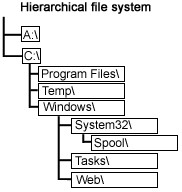
\includegraphics[width=0.27\linewidth]{hierarchy}
    \end{figure}
		
	\begin{choices}
        \CorrectChoice CorrectChoice depth-first traversal
        \choice Postorder depth-first traversal
        \choice Inorder depth-first traversal
        \choice Breadth-first traversal
	\end{choices}
\end{parts}

\newpage

\titledquestion{Tree Properties}

Answer the following questions for the tree shown below \textbf{according to  the definition specified in the lecture slides}. Please specify:

\begin{center}
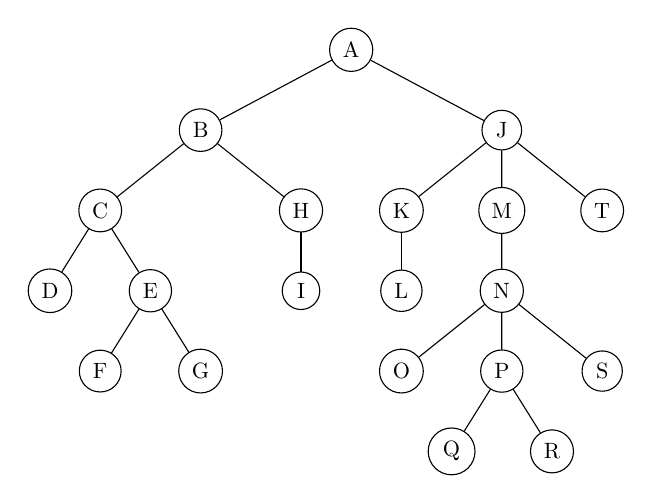
\begin{tikzpicture}[scale=0.85, every node/.style={scale=0.8}]
    \node [circle,draw] {A}
    child {node [circle,draw] {B}
        child {node [circle,draw] {C}
            child {node [circle,draw] {D}}
            child {node [circle,draw] {E}
                child {node [circle,draw] {F}}
                child {node [circle,draw] {G}}
            }
        }
        child [missing] {}
        child {node [circle,draw] {H}
            child {node [circle,draw] {I}}
        }
    }	
    child [missing] {}	
    child [missing] {}	
    child {node [circle,draw] {J}
        child {node [circle,draw] {K}
            child {node [circle,draw] {L}}
        }
        child {node [circle,draw] {M}
            child {node [circle,draw] {N}
                child {node [circle,draw] {O}}
                child {node [circle,draw] {P}
                    child {node [circle,draw] {Q}}
                    child {node [circle,draw] {R}}	
                }
                child {node [circle,draw] {S}}
            }
        }
        child {node [circle,draw] {T}}
    };
\end{tikzpicture}
\end{center}

\begin{parts}
    \part[2] The \textbf{children} of the \textbf{root node} with their \textbf{degree} respectively.
    \begin{solution}
        %%%%%%%%%%%%%%%%%%%%%%%%%%%%%%%%%%%%%%%%%%%%%%%%%
        % Replace `\vspace{2in}' with your answer.
        %\vspace{1in}
        B, J

        deg(B)=2, deg(J)=3
        %%%%%%%%%%%%%%%%%%%%%%%%%%%%%%%%%%%%%%%%%%%%%%%%%
    \end{solution}
    \part[2] All \textbf{leaf nodes} in the forest with their \textbf{depth} if we remove A and the node with the lexicographically smallest character in a tree is taken as the root node.
    \begin{solution}
        %%%%%%%%%%%%%%%%%%%%%%%%%%%%%%%%%%%%%%%%%%%%%%%%%
        % Replace `\vspace{2in}' with your answer.
        %\vspace{1in}
        D, F, G, I, L, O, Q, R, S, T

        height(T) = 1

        height(D) = height(I) = height(L) = 2

        height(F) = height(G) = height(O) = height(S) = 3

        height(Q) = height(R) = 4
        %%%%%%%%%%%%%%%%%%%%%%%%%%%%%%%%%%%%%%%%%%%%%%%%%
    \end{solution}
    \part[2] The \textbf{height} of the tree.
    \begin{solution}
        %%%%%%%%%%%%%%%%%%%%%%%%%%%%%%%%%%%%%%%%%%%%%%%%%
        % Replace `\vspace{2in}' with your answer.
        %\vspace{1in}
        height = max\{depth(v) | v \(\in\) V\} = 5

        so height = 5
        %%%%%%%%%%%%%%%%%%%%%%%%%%%%%%%%%%%%%%%%%%%%%%%%%
    \end{solution}

    \newpage

    \part[2] The \textbf{ancestors} of R. 
    \begin{solution}
        %%%%%%%%%%%%%%%%%%%%%%%%%%%%%%%%%%%%%%%%%%%%%%%%%
        % Replace `\vspace{2in}' with your answer.
        %\vspace{1in}
        R, P, N, M, J, A
        %%%%%%%%%%%%%%%%%%%%%%%%%%%%%%%%%%%%%%%%%%%%%%%%%
    \end{solution}
    \part[2] The \textbf{descendants} of L.
    \begin{solution}
        %%%%%%%%%%%%%%%%%%%%%%%%%%%%%%%%%%%%%%%%%%%%%%%%%
        % Replace `\vspace{2in}' with your answer.
        %\vspace{1in}
        L
        %%%%%%%%%%%%%%%%%%%%%%%%%%%%%%%%%%%%%%%%%%%%%%%%%
    \end{solution}
    \part[2] The \textbf{path} from E to S.
    \begin{solution}
        %%%%%%%%%%%%%%%%%%%%%%%%%%%%%%%%%%%%%%%%%%%%%%%%%
        % Replace `\vspace{2in}' with your answer.
        %\vspace{1in}
        \(E \to C \to B \to A \to J \to M \to N \to S\)
        %%%%%%%%%%%%%%%%%%%%%%%%%%%%%%%%%%%%%%%%%%%%%%%%%
    \end{solution}
\end{parts}

\newpage

\titledquestion{Tree Structure and Traversal}

Answer the following questions for the tree shown below \textbf{according to  the definition specified in the lecture slides}.

Note: Form your answer in the following steps.
\begin{enumerate}[1.]
    \item Decide on an appropriate \textbf{data structure} to implement the traversal.
    \item When you are pushing the children of a node into a \textbf{queue}, please push them alphabetically; when you are pushing the children of a node into a \textbf{stack}, please push them in a reversely alphabetical order.
    \item \textbf{Show all current elements in your data structure at each step} clearly. \textbf{Popping a node} or \textbf{pushing a sequence of children} can be considered as one single step.
    \item \textbf{Write down your traversal sequence} i.e. the order that you pop elements out of the data structure.
\end{enumerate}

Please refer to the examples displayed in the lecture slide for detailed implementation of traversal in a tree using the data structure.

\begin{parts}
    \part[4] Use stack to run \textbf{Preorder Depth First Traversal} in the tree with root E and you should fill stack step by step and then write down the traversal sequence. 
    \begin{center}
        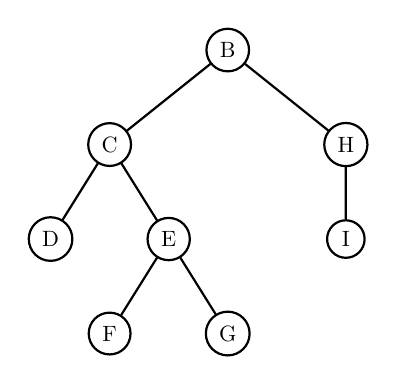
\begin{tikzpicture}[thick,scale=1.0, every node/.style={scale=0.8}]
            \node [circle,draw] {B}
            child {node [circle,draw] {C}
                    child {node [circle,draw] {D}}
                    child {node [circle,draw] {E}
                        child {node [circle,draw] {F}}
                        child {node [circle,draw] {G}}
                    }
            }	
            child [missing] {}
            child {node [circle,draw] {H}
                child {node [circle,draw] {I}}
            };
        \end{tikzpicture}
    \end{center}

    \begin{solution}

        \begin{minipage}{.14\linewidth}
            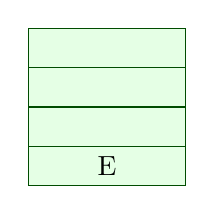
\begin{tikzpicture}[scale=0.5]
                \cell{}
                \cell{}
                \cell{}
                \cell{E}
            \end{tikzpicture}
        \end{minipage}
        $\to$
        \begin{minipage}{.14\linewidth}
            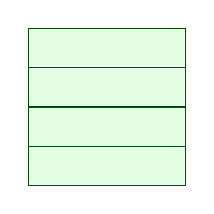
\begin{tikzpicture}[scale=0.5]
                \cell{}
                \cell{}
                \cell{}
                \cell{}
            \end{tikzpicture}
        \end{minipage}
        $\to$
        \begin{minipage}{.14\linewidth}
            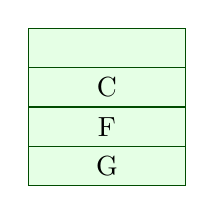
\begin{tikzpicture}[scale=0.5]
                \cell{}
                \cell{C}
                \cell{F}
                \cell{G}
            \end{tikzpicture}
        \end{minipage}
        $\to$
        \begin{minipage}{.14\linewidth}
            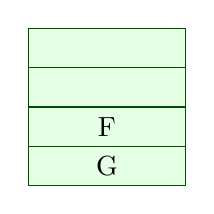
\begin{tikzpicture}[scale=0.5]
                \cell{}
                \cell{}
                \cell{F}
                \cell{G}
            \end{tikzpicture}
        \end{minipage}
        $\to$
        \begin{minipage}{.14\linewidth}
            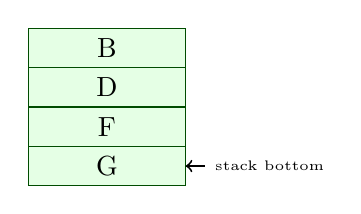
\begin{tikzpicture}[scale=0.5]
                \cell{B}
                \cell{D}
                \cell{F}
                \cell{G}\cellptr{\tiny {stack bottom}}
            \end{tikzpicture}
        \end{minipage}
        $\to$

        \begin{minipage}{.14\linewidth}
            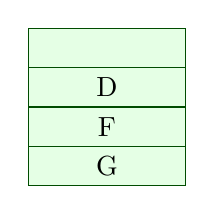
\begin{tikzpicture}[scale=0.5]
                \cell{}
                \cell{D}
                \cell{F}
                \cell{G}
            \end{tikzpicture}
        \end{minipage}
        $\to$
        \begin{minipage}{.14\linewidth}
            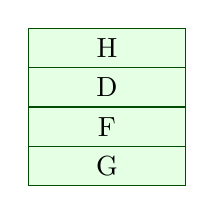
\begin{tikzpicture}[scale=0.5]
                \cell{H}
                \cell{D}
                \cell{F}
                \cell{G}
            \end{tikzpicture}
        \end{minipage}
        $\to$
        \begin{minipage}{.14\linewidth}
            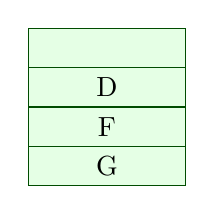
\begin{tikzpicture}[scale=0.5]
                \cell{}
                \cell{D}
                \cell{F}
                \cell{G}
            \end{tikzpicture}
        \end{minipage}
        $\to$
        \begin{minipage}{.14\linewidth}
            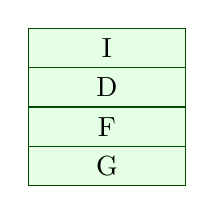
\begin{tikzpicture}[scale=0.5]
                \cell{I}
                \cell{D}
                \cell{F}
                \cell{G}
            \end{tikzpicture}
        \end{minipage}
        $\to$
        \begin{minipage}{.14\linewidth}
            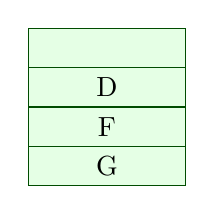
\begin{tikzpicture}[scale=0.5]
                \cell{}
                \cell{D}
                \cell{F}
                \cell{G} 
            \end{tikzpicture}
        \end{minipage}
        $\to$

        \begin{minipage}{.14\linewidth}
            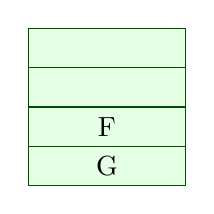
\begin{tikzpicture}[scale=0.5]
                \cell{}
                \cell{}
                \cell{F}
                \cell{G}
            \end{tikzpicture}
        \end{minipage}
        $\to$
        \begin{minipage}{.14\linewidth}
            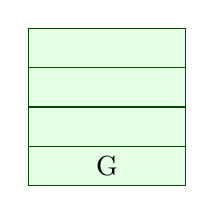
\begin{tikzpicture}[scale=0.5]
                \cell{}
                \cell{}
                \cell{}
                \cell{G}
            \end{tikzpicture}
        \end{minipage}
        $\to$
        \begin{minipage}{.14\linewidth}
            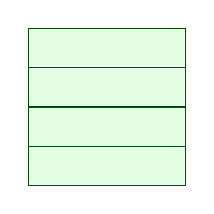
\begin{tikzpicture}[scale=0.5]
                \cell{}
                \cell{}
                \cell{}
                \cell{}
            \end{tikzpicture}
        \end{minipage}
        $\to$
        \begin{minipage}{.14\linewidth}
            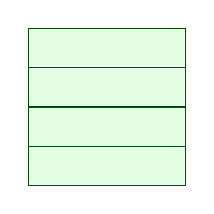
\begin{tikzpicture}[scale=0.5]
                \cell{}
                \cell{}
                \cell{}
                \cell{}
            \end{tikzpicture}
        \end{minipage}
        $\to$
        \begin{minipage}{.14\linewidth}
            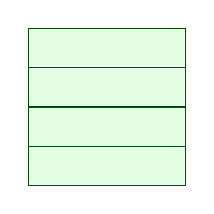
\begin{tikzpicture}[scale=0.5]
                \cell{}
                \cell{}
                \cell{}
                \cell{}
            \end{tikzpicture}
        \end{minipage}

        Traversal Sequence: E, C, B, H, I, D, F, G
    \end{solution}
    
    \newpage
    \part[4] Use queue to run \textbf{Breadth First Traversal} in the tree with root P and you should fill queue step by step and then write down the traversal sequence. 

    \begin{center}
        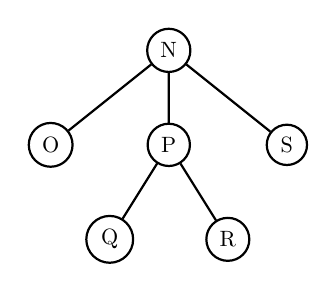
\begin{tikzpicture}
            [thick,scale=1, every node/.style={scale=0.8}]
            \node [circle,draw] {N}
                child {node [circle,draw] {O}}
                child {node [circle,draw] {P}
                    child {node [circle,draw] {Q}}
                    child {node [circle,draw] {R}}	
                }
                child {node [circle,draw] {S}};
        \end{tikzpicture}
    \end{center}
    \begin{solution}\par
        \begin{minipage}{.14\linewidth}
            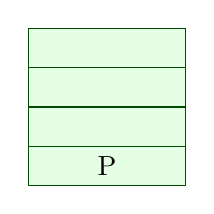
\begin{tikzpicture}[scale=0.5]
                \cell{}
                \cell{}
                \cell{}
                \cell{P}
            \end{tikzpicture}
        \end{minipage}
        $\to$
        \begin{minipage}{.14\linewidth}
            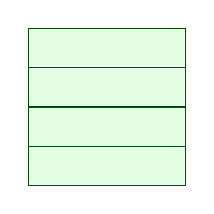
\begin{tikzpicture}[scale=0.5]
                \cell{}
                \cell{}
                \cell{}
                \cell{}
            \end{tikzpicture}
        \end{minipage}
        $\to$
        \begin{minipage}{.14\linewidth}
            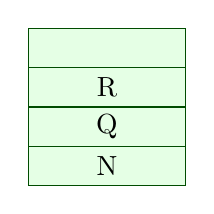
\begin{tikzpicture}[scale=0.5]
                \cell{}
                \cell{R}
                \cell{Q}
                \cell{N}
            \end{tikzpicture}
        \end{minipage}
        $\to$
        \begin{minipage}{.14\linewidth}
            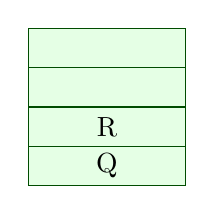
\begin{tikzpicture}[scale=0.5]
                \cell{}
                \cell{}
                \cell{R}
                \cell{Q}
            \end{tikzpicture}
        \end{minipage}
        $\to$
        \begin{minipage}{.14\linewidth}
            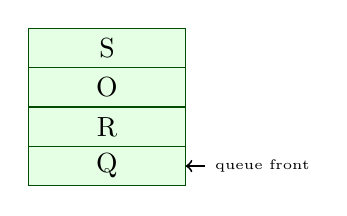
\begin{tikzpicture}[scale=0.5]
                \cell{S}
                \cell{O}
                \cell{R}
                \cell{Q}\cellptr{\tiny {queue front}}
            \end{tikzpicture}
        \end{minipage}
        $\to$

        \begin{minipage}{.14\linewidth}
            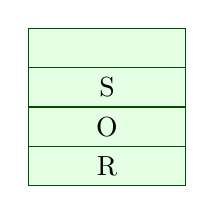
\begin{tikzpicture}[scale=0.5]
                \cell{}
                \cell{S}
                \cell{O}
                \cell{R}
            \end{tikzpicture}
        \end{minipage}
        $\to$
        \begin{minipage}{.14\linewidth}
            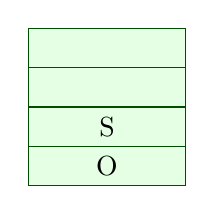
\begin{tikzpicture}[scale=0.5]
                \cell{}
                \cell{}
                \cell{S}
                \cell{O}
            \end{tikzpicture}
        \end{minipage}
        $\to$
        \begin{minipage}{.14\linewidth}
            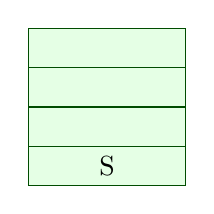
\begin{tikzpicture}[scale=0.5]
                \cell{}
                \cell{}
                \cell{}
                \cell{S}
            \end{tikzpicture}
        \end{minipage}
        $\to$
        \begin{minipage}{.14\linewidth}
            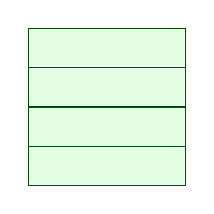
\begin{tikzpicture}[scale=0.5]
                \cell{}
                \cell{}
                \cell{}
                \cell{}
            \end{tikzpicture}
        \end{minipage}
        $\to$
        \begin{minipage}{.14\linewidth}
            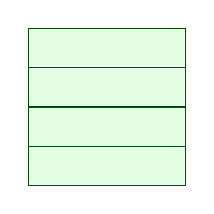
\begin{tikzpicture}[scale=0.5]
                \cell{}
                \cell{}
                \cell{}
                \cell{} 
            \end{tikzpicture}
        \end{minipage}

        Traversal Sequence: P, N, Q, R, O, S
    \end{solution}

\end{parts}

\newpage

\titledquestion{Recurrence Relations}

For each question, find the asymptotic order of growth of $T(n)$ i.e. find a function $g$ such that $T(n) = O(g(n))$. You may ignore any issue arising from whether a number is an integer. You can make use of the Master Theorem, Recursion Tree or other reasonable approaches to solve the following recurrence relations.

\begin{parts}
    \part[4] $T(n) = 4T(n/2) + 2^4\cdot\sqrt{n}$ and $T(0) = 1$.
    \begin{solution}
        %%%%%%%%%%%%%%%%%%%%%%%%%%%%%%%%%%%%%%%%%%%%%%%%%
        % Replace `\vspace{2in}' with your answer.
        % \vspace{2.5in}
        by the Master Theorem,

        $ a = 4, b = 2 , and \ 2^4 \sqrt{n} = \Theta(\sqrt{n}), so \ d = \frac{1}{2}$

        $ log_ba = log_24 = 2 > d = \frac{1}{2}$

        so $ T(n) = O(n^{log_ba}) = O(n^2)$

        $ T(n) = O(n^2) , g(n) = n^2$
        %%%%%%%%%%%%%%%%%%%%%%%%%%%%%%%%%%%%%%%%%%%%%%%%%
    \end{solution}
    \part[4] $T(n) = T(n / 4) + T(n / 2) + c \cdot n ^ 2$ and $T(0) = 1$, $c$ is a positive constant.
    \begin{solution}
        %%%%%%%%%%%%%%%%%%%%%%%%%%%%%%%%%%%%%%%%%%%%%%%%%
        % Replace `\vspace{2in}' with your answer.
        %\vspace{2.5in}
        set $f_k$ be k-th the element in the fabonacci sequence
        
        which $f_0 = 1, f_1 = 1, f_n = f_{n-2}+f_{n-1} (n\geq 2)$

        and since $f_1 = 1 < 2^1, f_2 = 2 < 2^2 , f_n = f_{n-2}+f_{n-1}, 2^n = 2^{n-1} + 2^{n-1}$

        so $f_k \leq 2^k$

        since $T(n)=T(\frac{n}{2})+T(\frac{n}{4})+c \cdot n^2=f_0 \cdot T(\frac{n}{2})+f_0 \cdot T(\frac{n}{4})+f_1 \cdot c \cdot n^2$
        
        $T(\frac{n}{2})=T(\frac{n}{4})+T(\frac{n}{8})+f_1 \cdot c \cdot (\frac{n}{2})^2$

        so $T(n)=(f_0+f_1) \cdot T(\frac{n}{4})+f_1 \cdot T(\frac{n}{8})+f_0 \cdot c \cdot n^2+f_1 \cdot c \cdot (\frac{n}{2})^2=$

        $=f_2 \cdot T(\frac{n}{4})+f_1 \cdot T(\frac{n}{8})+f_0 \cdot c \cdot n^2+f_1 \cdot c \cdot (\frac{n}{2})^2$


        $\cdots$

        $=f_i\cdot T(\frac{n}{2^i})+f_{i-1}\cdot T(\frac{n}{2^{i+1}})+\sum_{k=0}^{i-1} f_k \cdot c \cdot (\frac{n}{2^k})^2$
        
        $=f_i \cdot \{ T(\frac{n}{2^{i+1}})+T(\frac{n}{2^{i+2}})+c\cdot (\frac{n}{2^i})^2 \} +f_{i-1}\cdot T(\frac{n}{2^{i+1}})+\sum_{k=0}^{i-1} f_k \cdot c \cdot (\frac{n}{2^k})^2$

        $=f_{i+1}\cdot T(\frac{n}{2^{i+1}})+f_{i}\cdot T(\frac{n}{2^{i+2}})+\sum_{k=0}^{i} f_k \cdot c \cdot (\frac{n}{2^k})^2$


        $\cdots$

        so $T(n) \leq 1 + 1 + \sum_{k=01}^{\lceil logn \rceil} f_k \cdot c \cdot (\frac{n}{2^k})^2$

        and since we have proved above $f_k \leq 2^k$

        so $T(n) \leq c \cdot \sum_{k=0}^{\lceil logn \rceil} 2^k*\frac{n^2}{(2^k)^2}$

        $T(n) \leq c \cdot n^2 \cdot \sum_{k=0}^{\lceil logn \rceil} \frac{1}{2^k} \leq 2c \cdot n^2$

        $T(n) \leq 2c\cdot n^2$

        so above all, $T(n)=O(n^2),g(n)=n^2$
        
        %%%%%%%%%%%%%%%%%%%%%%%%%%%%%%%%%%%%%%%%%%%%%%%%%
    \end{solution}
    
    \newpage

    \part[4] $T(n) = T(\sqrt{n}) + 1$ and $T(2)=T(1)=1$.
    \begin{solution}
        %%%%%%%%%%%%%%%%%%%%%%%%%%%%%%%%%%%%%%%%%%%%%%%%%
        % Replace `\vspace{2in}' with your answer.
        %\vspace{3in}
        let $ n^{\frac{1}{2^k}} \leq 2$

        so $ 2^k \geq log_2n$

        so $ k \geq \lceil log_2(log_2n) \rceil$

        since T(2)=T(1)=1

        so $T(n)=T(\sqrt{n})+1=T(n^\frac{1}{4})+2=\cdots=T(n^{\frac{1}{2^k}})+k \leq 1+k$

        so $T(n)=O(k)=O(log_2log_2n)$
        
        so above all, $T(n)=O(loglogn), g(n)=loglogn$
        %%%%%%%%%%%%%%%%%%%%%%%%%%%%%%%%%%%%%%%%%%%%%%%%%
    \end{solution}
\end{parts}

\newpage

\titledquestion{Maximum Contiguous Subsequence Sum}[8]

Given an array $\langle a_1,\cdots,a_n\rangle$ of length $n$ with both \textbf{positive} and \textbf{negative} elements, we will design a \textbf{divide and conquer} algorithm to find the maximum contiguous subsequence sum of $a$. We say $m$ is the  maximum contiguous subsequence sum of $a$ such that for any integer pair $(l,r)$ ($1 \le l \le r \le n$), 
$$
m \ge \sum_{i = l} ^ r a_i.
$$
The time complexity should be $\Theta(n \log n)$.
\begin{solution}
%%%%%%%%%%%%%%%%%%%%%%%%%%%%%%%%%%%%%%%%%%%%%%%%%
% Replace `\vspace{2in}' with your answer.
%\vspace{6in}
\paragraph{Algorithm Design:} 
after divide the sequence into two parts from the middle

the maximum contiguous subsequence may have three possible location distributions
\begin{enumerate}
	\item the whole subsequence is in the left part
	\item the whole subsequence is in the right part
	\item the subsequence is in both left part and right part, and it get through the middle
\end{enumerate}

\iffalse
so we need to maintain four variables during the divide and conquer

they are the $maxn, lmax, rmax, sum$

\begin{itemize}
	\item $sum$ , it is the easist one, just the sum of all numbers of the subsequence,
	and we can maintain it by adding left-subsequence's $sum+$ right-subsequence's $sum$

	\item $lmax$, it is the maximum contiguous subsequence start from the left point of the subsequence,
	there are two possibilites:
	
	\begin{itemize}
		\item it may be the left subsequence's $lmax$
		\item it may be the whole left sequence with part of the right-subsequence
	\end{itemize}
	
	and we can maintain it by acquiring the maximum one bewteen left-subsequence's $lmax$ and (left-subsequence's $sum+$ right-subsequence's $lmax$	)

	\item $rmax$, it is similar to the $lmax$,
	so just let $rmax=max\{$ right-subsequence's $rmax$ , (right-subsequence's $sum+$ left-subsequence's $rmax)\}$
	
	\item $maxn$, it is the maximum contiguous subsequence of the whole subsequence,
	from the discuss at the begining, we can maintain it by letting 
	
	$maxn=max\{ left-subsequence's \ maxn , right-subsequence's \ maxn , left-subsequence's \ rmax \ +\  right-subsequence's\ lmax\}$
	
\end{itemize}

and at last, we only need to know the $maxn$ of the whole sequence.

\fi

and for the first two situations,
for the left-subsequence and right-subsequence, they have the samilar situation above

and for the third situation, we just need to start at the middle point, expand to the left and right respectively,
and find the maximum contiguous subsequence respectively, then sum them up.

so we can recursively divide and conquer the problem
\paragraph{Pseudocode :}
$left$ and $right$ are indecies of the leftmost and rightmost elements in given array $a$ respectively.
\begin{algorithm}[H]
	\begin{algorithmic}[1]
		\Function {get\_max\_contiguous\_subsequence}{$a$, $left$, $right$}
		\If {$right == left$} 
		\State \Return max(0,a[left])
		\EndIf
		\State $mid\gets \lfloor (left + right)/2 \rfloor$
		\State $left\_subsequence\gets get\_max\_contiguous\_subsequence(a,left,mid)$
		\State $right\_subsequence\gets get\_max\_contiguous\_subsequence(a,mid+1,right)$

		define sum=0,lmax=0

		for(i from mid to left):

		\ \ \ \ \	sum+=a[i]

		\ \ \ \ \ 	lmax=max(lmax,sum)

		similarly, define sum=0,rmax=0

		for(i from (mid+1) to right):

		\ \ \ \ \ 	sum+=a[i]

		\ \ \ \ \ 	rmax=max(rmax,sum)
		\State $mid\_subsequence\gets (lmax+rmax)$

		\State $maxn\gets max\{left\_subsequence, right\_subsequence, mid\_subsequence\}$
		\State \Return maxn
		\EndFunction
	\end{algorithmic}
\end{algorithm}

\paragraph{Time Complexity Analysis:}
During each recursion, the calculation of $mid$ and comparison can be done in constant time, 
and getting the $lmax$ and $rmax$ takes the time of the sequence's length, which is exactly $\Theta(n)$. We will take both half part of the sequence, thus there are two times of each subproblem.
$$T(n) = 2\cdot T(\frac{n}{2})+\Theta(n)$$
Therefore, by the Master Theorem,

$a=2,b=2,\log_{b}{a}=1=d$, so $T(n) = \Theta(nlogn)$.
%%%%%%%%%%%%%%%%%%%%%%%%%%%%%%%%%%%%%%%%%%%%%%%%%
\end{solution}

\newpage

\titledquestion{\(k\)-th Minimal Value}

Given an array \(\langle a_1,\cdots,a_n\rangle\) of length \(n\) with \emph{distinct} elements and an integer \(k\in[1,n]\), we will design an algorithm to find the \(k\)-th minimal value of \(a\). We say \(a_x\) is the \(k\)-th minimal value of \(a\) if there are exactly \(k-1\) elements in \(a\) that are less than \(a_x\), i.e.
\[\left|\left\{i\mid a_i<a_x\right\}\right|=k-1.\]
Consider making use of the `\textbf{partition}' procedure in quick-sort. The function has the signature
\begin{cpp}
  int partition(int a[], int l, int r);
\end{cpp}
which processes the subarray \(\langle a_l,\cdots,a_r\rangle\). It will choose a pivot from the subarray, place all the elements that are less than the pivot before it, and place all the elements that are greater than the pivot after it. After that, the index of the pivot is returned.

Our algorithm to find the \(k\)-th minimal value is implemented below.
\begin{cpp}
  // returns the k-th minimal value in the subarray a[l],...,a[r].
  int kth_min(int a[], int l, int r, int k) {
    auto pos = partition(a, l, r), num = pos - l + 1;
    if (num == k)
      return a[pos];
    else if (num > k)
      return kth_min(____a, l, pos - 1, k____________);
    else
      return kth_min(____a, pos + 1, r, k - num______);
  }
\end{cpp}
By calling \lstinline{kth_min(a, 1, n, k)} we will get the answer.

\begin{parts}
  \part[2] Fill in the blanks in the code snippet above.
  \part[3] What's the time complexity of our algorithm in the \textbf{worst case}? Please answer in the form of \(\Theta(\cdot)\) and fully justify your answer.
  \begin{solution}
    %%%%%%%%%%%%%%%%%%%%%%%%%%%%%%%%%%%%%%%%%%%%%%%%%
    % Replace `\vspace{2in}' with your answer.
    %\vspace{2in}
    let \(T(n)\) be the time complexity with \(n\) elements in the array
    
    for the worst case
    
    \(1\.\) if  \(k \leq \frac{n}{2}\) ,the partition always choose the pivot at the end of the sub-array

    \(T(n) = T(n-1) + \Theta(n)\)

    \(T(n-1) = T(n-2) + \Theta(n-1)\)

    \(...\)

    and \(T(k) = 1\)

    so \(T(n) = T(k) + n + (n-1) + ... + (k+1) = \frac{n^2+n-k^2-k-2}{2} = \Theta(\frac{3}{8}n^2 + \frac{n}{4} +1)\)
    
    \(T(n) = \Theta(n^2)\)

    \(2\.\) if \(k > \frac{n}{2}\) ,the partition always choose the pivot at the begin of the sub-array

    \(T(n) = T(n-1) + \Theta(n)\)

    \(T(n-1) = T(n-2) + \Theta(n-1)\)

    \(...\)

    and \(T(n-k+1) = 1\)

    so \(T(n) = T(n-k+1) + n + (n-1) + ... + (n-k) = nk - \frac{k^2}{2} = \Theta(\frac{n^2}{2})\)
    
    \(T(n) = \Theta(n^2)\)

    so above all, the worst case of the time complexity is \(\Theta(n^2)\)

    %%%%%%%%%%%%%%%%%%%%%%%%%%%%%%%%%%%%%%%%%%%%%%%%%
  \end{solution}
\end{parts}

\end{questions}

\end{document}